\documentclass{csc_assignment4}
\usepackage[utf8]{inputenc}
\usepackage[letterpaper, portrait, margin=1in]{geometry}
\usepackage{calc}  % arithmetic in length parameters
\usepackage{enumitem}  % more control over list formatting
\usepackage{fancyhdr}  % simpler headers and footers
\usepackage{lastpage}  % for last page number
\usepackage{relsize}  % easier font size changes
\usepackage[normalem]{ulem}  % smarter underlining
\usepackage{url}  % verb-like typesetting of URLs
\usepackage{xfrac}  % nicer looking simple fractions for text and math
\usepackage{amsmath}
\usepackage{amssymb}
\usepackage{tikz}
\usepackage{algorithm}
\usepackage{algorithmic}
\usepackage{graphicx}
\usepackage{listings}
\graphicspath{{/}}
\usepackage[export]{adjustbox}
\usepackage{enumitem}
\usepackage{subcaption}

 \lstset{breaklines=true}

% ----------------------------------------------------------------
% TODO: Enter the assignment number, your name, and your student number below
% ----------------------------------------------------------------
\AssignmentName{Assignment 2}
\StudentName{Akhil Gupta}
\StudentNumber{1000357071}

% ----------------------------------------------------------------
\begin{document}
\begin{description}

\item[Q1.]
Interest Point Detection:
\begin{enumerate}[label=(\alph*)]
\item
\begin{lstlisting}[language=MATLAB]
function out = a2q1a(filename)
% read image and grayscale
im = imread(filename);
img = rgb2gray(im);
[img_height, img_width] = size(img);

% compute gradients Ix and Iy
[Ix, Iy] = imgradientxy(img);

% compute Ix^2, Iy^2, Ix * Iy
Ix2 = Ix.^2;
Iy2 = Iy.^2;
Ixy = Ix.*Iy;

% compute matrix M = [Ix2g, Ixyg; Ixyg, Iy2g];
gauss_filter = fspecial('gaussian');
Ix2g = conv2(Ix2, gauss_filter, 'same');
Iy2g = conv2(Iy2, gauss_filter, 'same');
Ixyg = conv2(Ixy, gauss_filter, 'same');

% compute R = det(M) - alpha*trace(M)^2
alpha = 0.04; 
Rmax = 0;
R = zeros(img_height, img_width);
det_M = Ix2g.*Iy2g - Ixyg.^2;
trace_M = Ix2g + Iy2g; 
R = det_M - alpha*((trace_M).^2);
Rmax = max(max(R));

% Non-maximum suppression
Res = zeros(img_height, img_width);
thresh = Rmax*0.028;
for row = 1:img_height
    for col = 1:img_width
        % check for local max
        if R(row,col) > thresh
            local_max = true;
            for n = row-1:row+1
                for m = col-1:col+1
                    if R(n, m) > R(row, col)
                        local_max = false;
                        break
                    end
                end
                if local_max == false
                    break
                end
            end
            if local_max == true
                Res(row,col) = 1;
            end
        end
    end
end

[cols, rows] = find(Res == 1);
imshow(img);
hold on;
plot(rows,cols,'r.');
end
\end{lstlisting}
\begin{figure}[h]
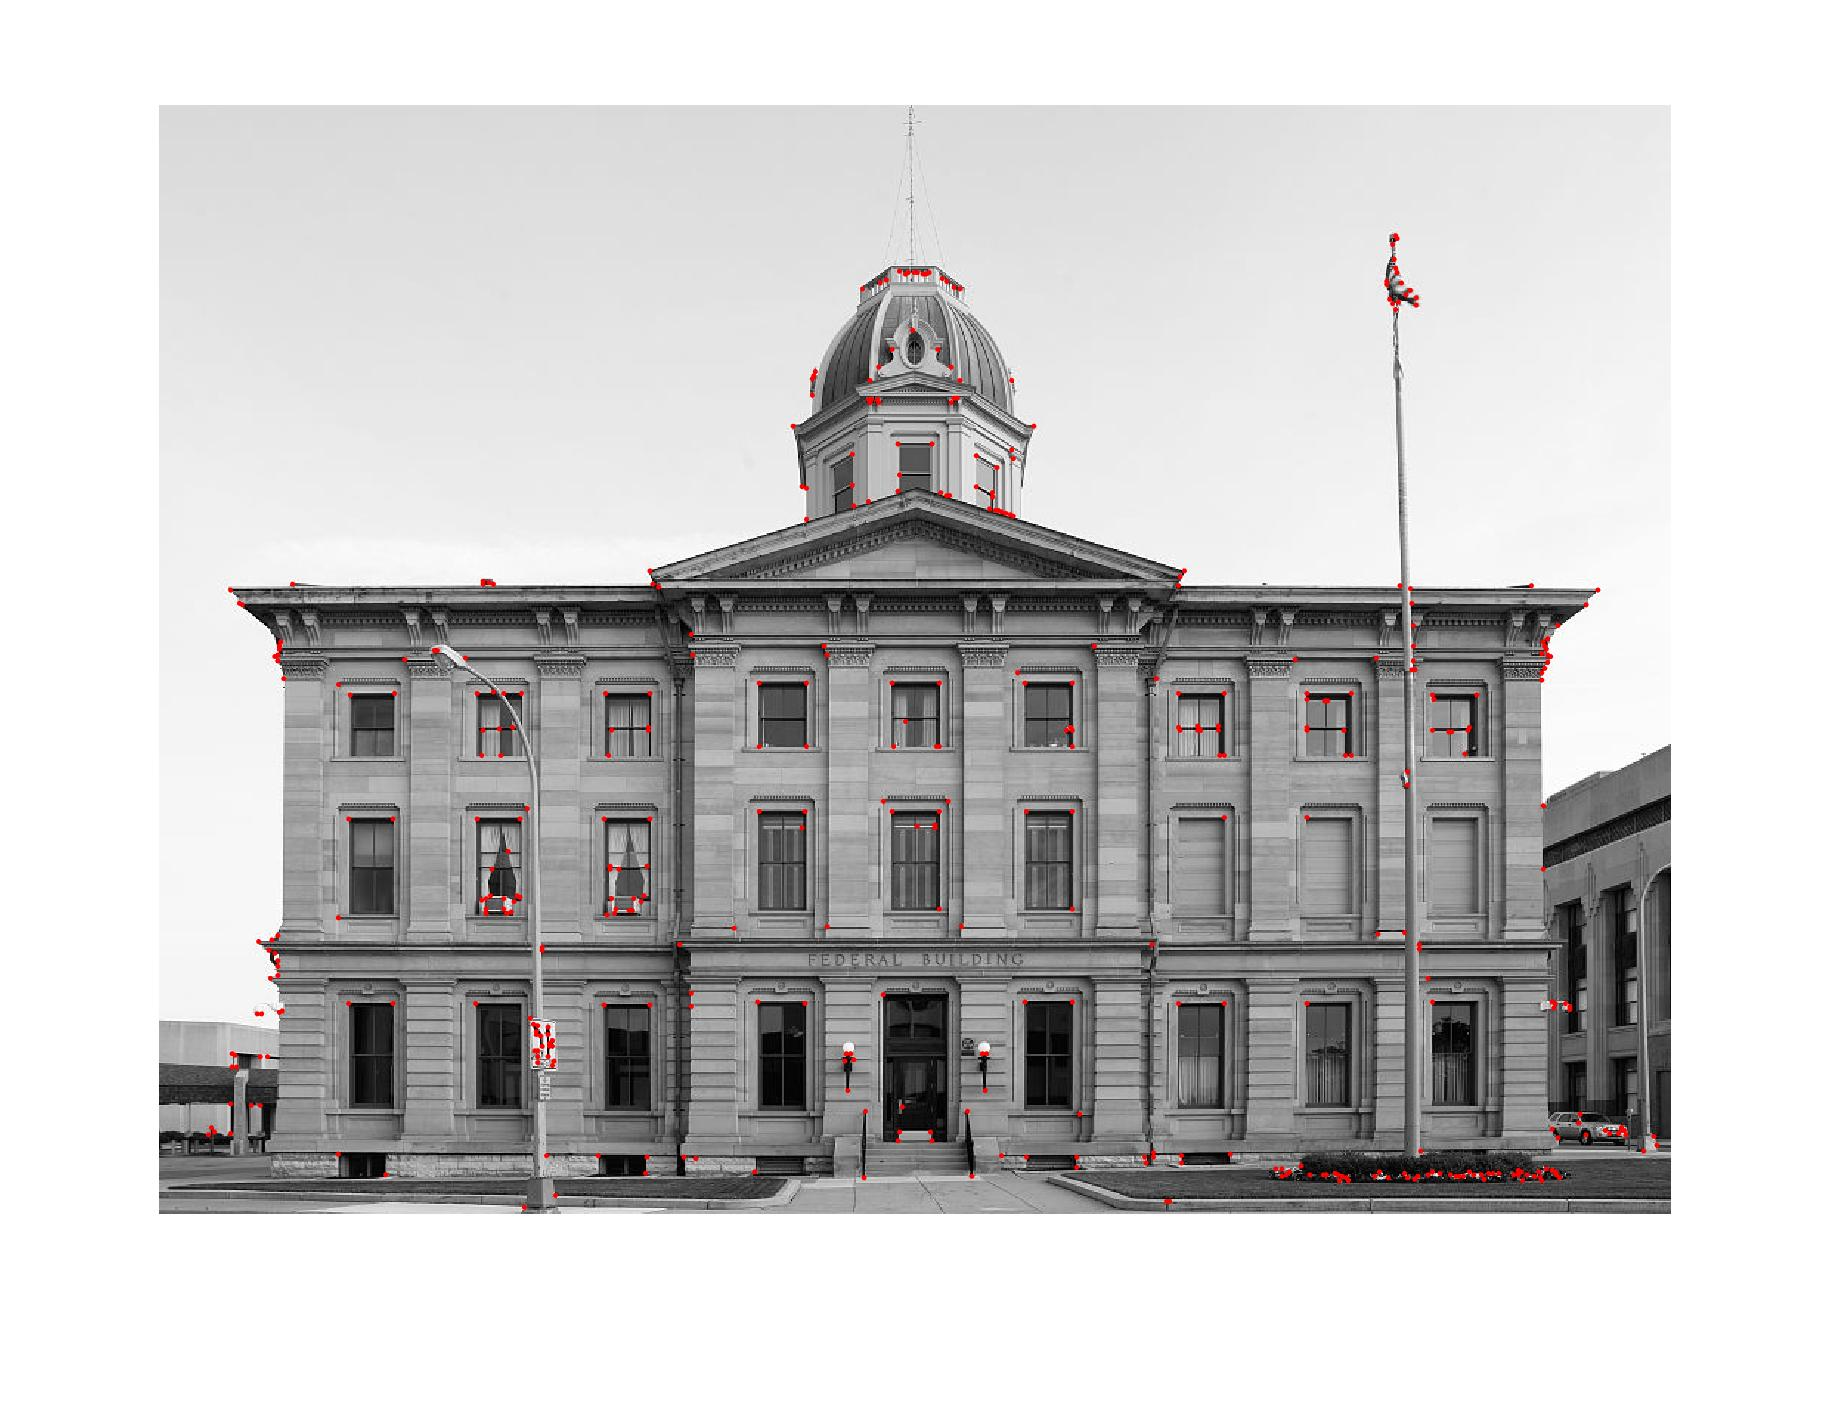
\includegraphics[width=0.8\textwidth, center]{harris_corners.jpg}
\vspace*{-20mm}
\caption{Harris Corner Detection run on building 1.jpg}
\end{figure}

\newpage
\item   
Pseudo-Code for Lowe's scale-invariant algorithm interest point detection: \begin{enumerate}
\item Compute a gaussian image pyramid: This step is used to find \textbf{scale invariant} interests points in each image independently. We do this by creating a gaussian pyramid that basically applies multiple gaussian filters one on top of the other at every scale of an image. That is, for scale = 1, the algorithm applies a gaussian filter of size $\sigma$, then $k\sigma$, $k^{2}\sigma$... where $k = 2^{1/s}$ where $s$ is the scale of the image. Each image is smoothed by a factor of $k$ more than the image below. Then we scale down the image by 1/2 so scale = 0.5, and again apply multiple gaussian filters one by one till we hit the next scale. Each scale is called an ``octave''. This creates our gaussian pyramid.
\item Compute Difference of Gaussians at every scale: This step is used to calculate the difference of gaussians that we calculated at each step in the step above. We calculate the difference of gaussians at each ``octave''/scale and between images within the same octave. So if we have 5 images in the first octave, we get 4 values for difference of gaussians. We do Difference of Gaussians rather than Laplacian of Gaussians as it computationally cheaper and DoG is a very good approximation of LoG.
\item Find local maxima in each scale: This step finds the local maxima in every octave. The local maxima are the interest points that we are looking for. These points are scale-invariant because we computed the gaussian image pyramid in step 1) that scales the images down. We also prune the mislabelled local maxima in order to get the true maximum. 
\end{enumerate}
\end{enumerate}

\item[Q2.]
\begin{enumerate}[label=(\alph*)]
\item Feature Extraction: 
\begin{lstlisting}[language=MATLAB]
% SIFT features for reference.png, test.png and test2.png
function out = a2q2a()
% read images and grayscale
im = imread('reference.png');
img = single(rgb2gray(im));

% get frames and descriptors for images
[f, d] = vl_sift(img);

% Plot images (used separate library for plotting because vl_plotframe caused errors)
imshow(im);
hold on;
h1 = plotsiftframe(f(:,1:100));
set(h1,'color','r','linewidth',1);
hold off;

end
\end{lstlisting}
***OUTPUT ON NEXT PAGE***
\begin{figure}
\vspace*{-25mm}

\includegraphics[width=0.7\textwidth, center]{reference_features.jpg}
\vspace*{-20mm}
\caption{Feature Extraction run on reference.png}
\vspace*{-22mm}
\end{figure}
\vspace*{-25mm}
\begin{figure}
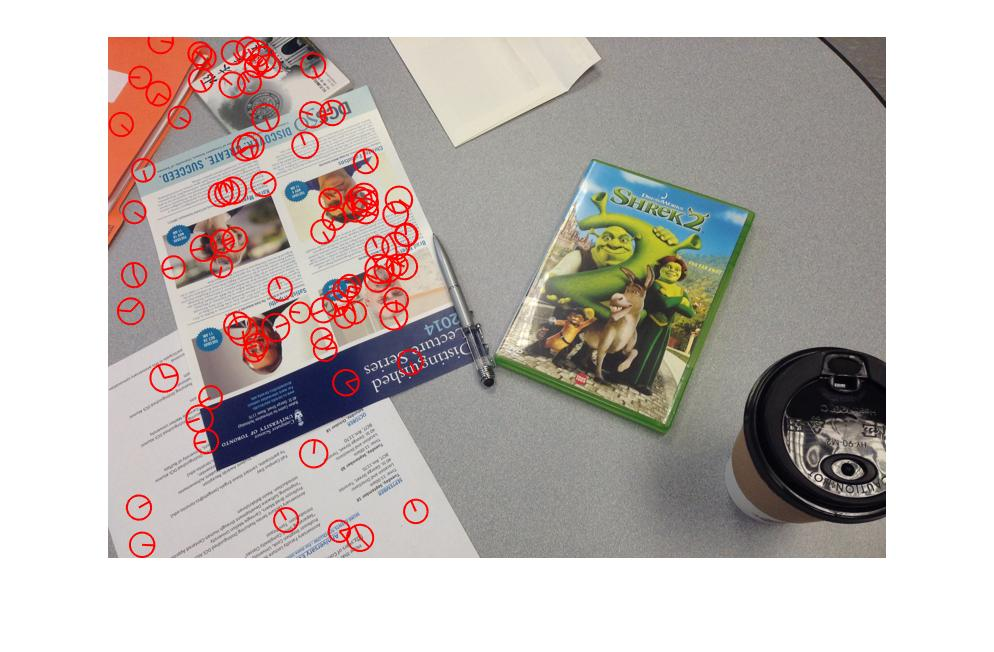
\includegraphics[width=0.7\textwidth, center]{test_features.jpg}
\vspace*{-14mm}
\caption{Feature Extraction run on test.png}
\end{figure}
\begin{figure}
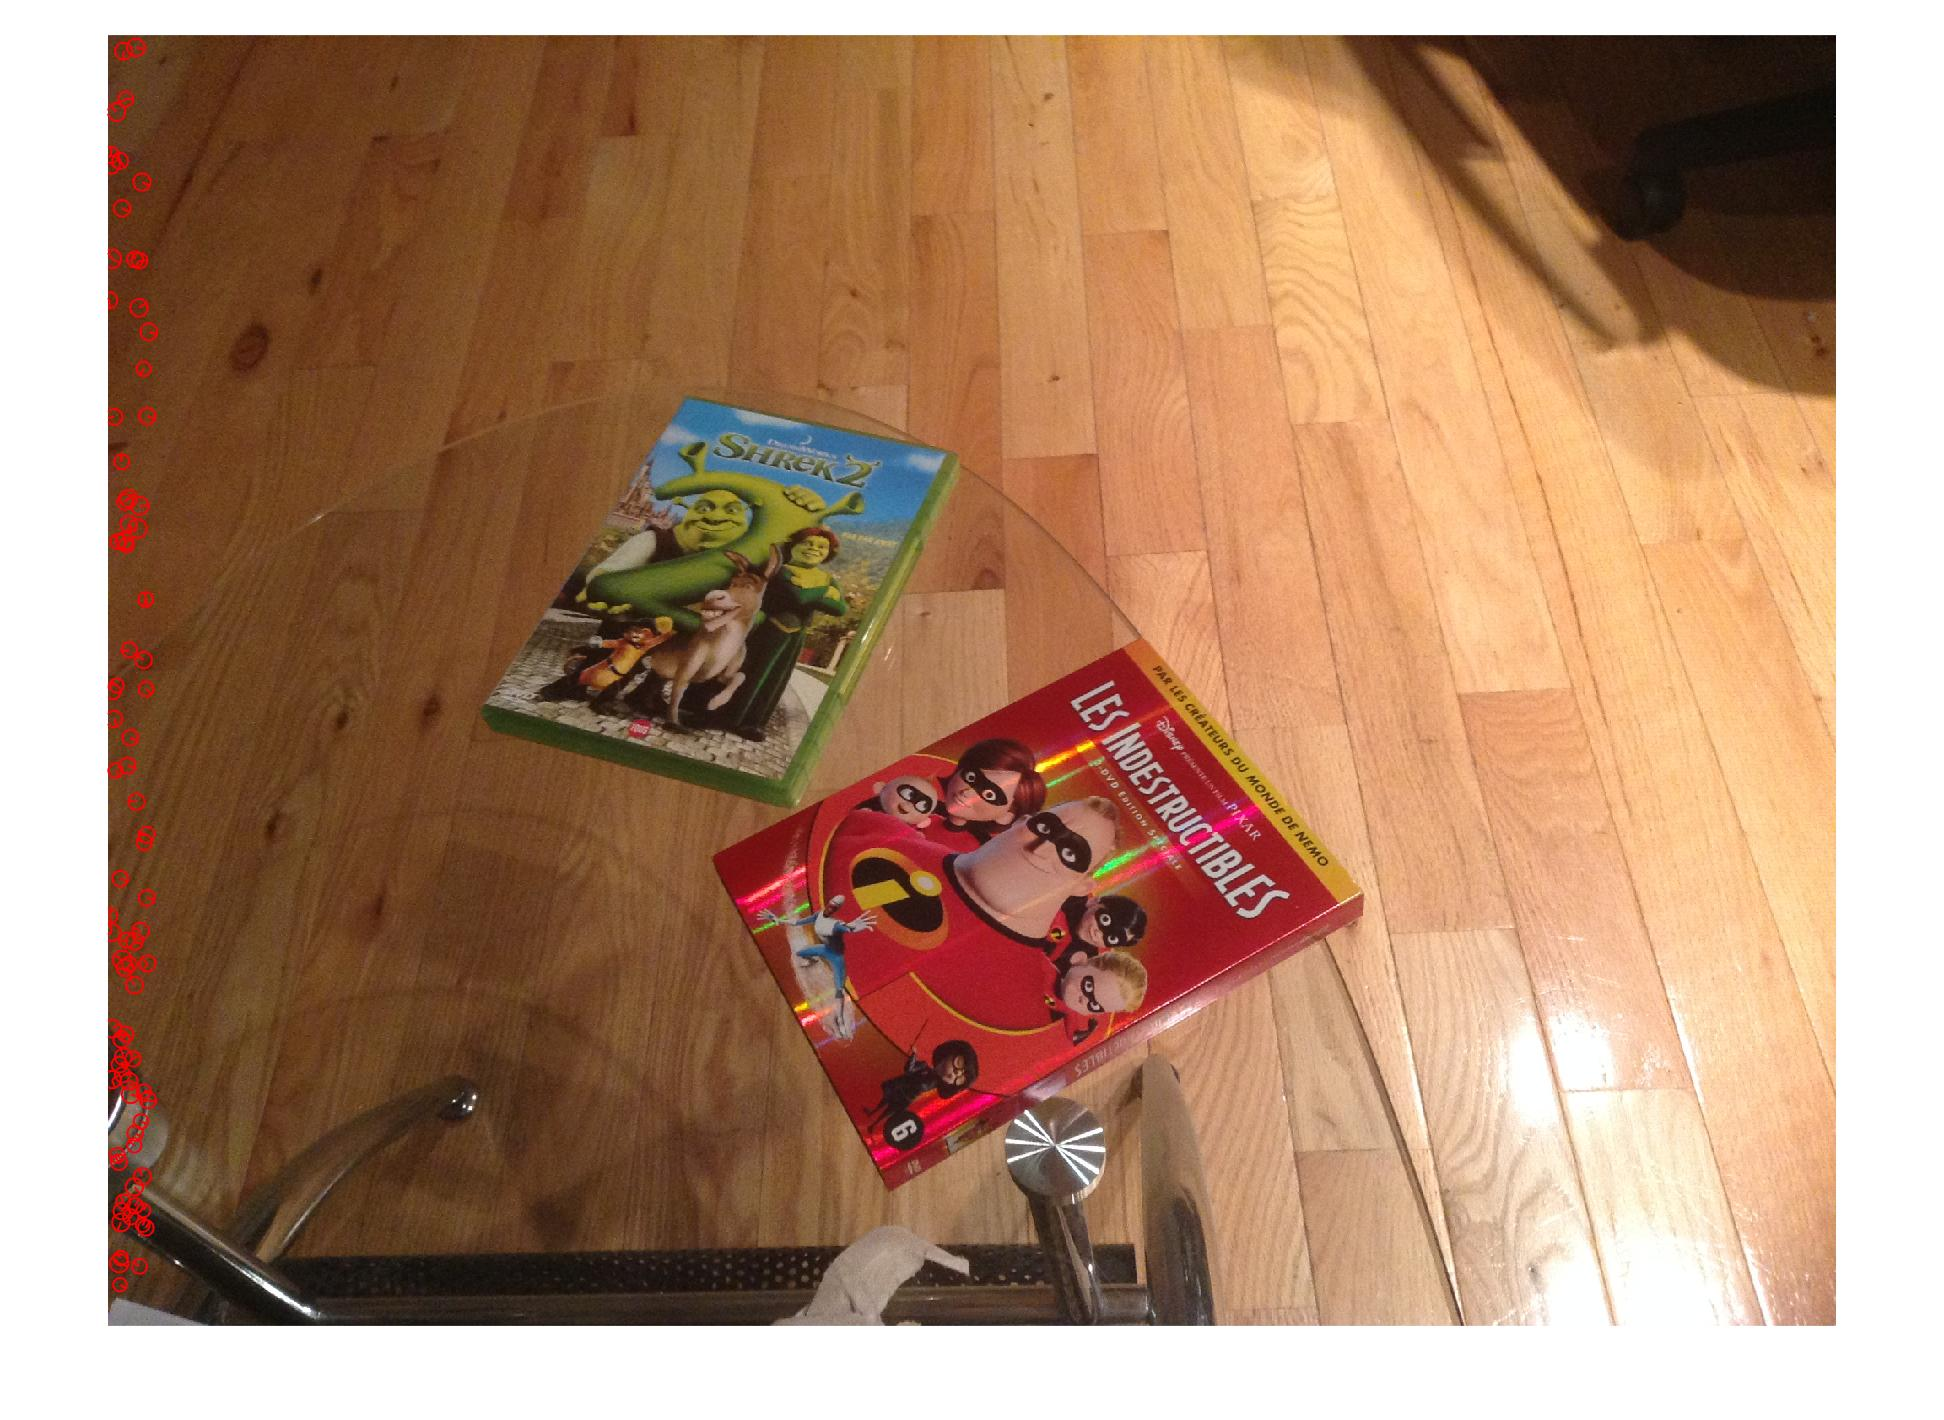
\includegraphics[width=0.7\textwidth, center]{test2_features.jpg}
\vspace*{-10mm}
\caption{Feature Extraction run on test2.png}
\end{figure}

\newpage
\item Matching: \\
In order to find the best feature matches for the features in refernce.png and features in test.png, we can apply the following simple algorithm discussed in lecture:
\begin{itemize}
\item First, we find extract a SIFT feature descriptor around each interest point (the interest points are calculated from Lowe's scale invariant interest point detection in Question 1.) Each descriptor has location, scale, orientation and the 128-dim feature vector. 
\item In order to perform matching, we match the extracted keypoints and their descriptors between pairs of images. To do that, we compute the euclidean distance between all the feature vectors combinations in both images. 
\item We pick one feature vector in the first image and find the closest and second closest match difference in the second image. To illustrate, if $f_{1}$ is a feature vector in the first image, and $f_{1}', ..., f_{k}'$ are the $k$-feature vectors in the second image, we compute $||f_{1} - f_{1}'||, ||f_{1} - f_{2}'||, ..., ||f_{1} - f_{k}'||$ and pick the first min distance and second min distance. 
\item We then compute the ratio between the closest and second closest match. $\phi_{i} = \frac{||f_{i} - f_{i}'*||}{||f_{i} - f_{i}'**||}$ where $f_{i}'*$ is the first closest match and $f_{i}'**$ is the second closest match. 
\item We usually threshold the ratio ($\phi_{i}$) at 0.8 to prevent from getting too many false positives or too many false negatives. 
\item Now, we can match features in our pair of images!
\end{itemize}
\newpage
\begin{lstlisting}[language=MATLAB]
% SIFT features for reference.png and test.png
function out = a2q2b()

% read images and grayscale
im_test = imread('test2.png');
img_test = single(rgb2gray(im_test));
im_ref = imread('reference.png');
img_ref = single(rgb2gray(im_test));

% get frames and descriptors for images
[f_test, d_test] = vl_sift(img_test);
[f_ref, d_ref] = vl_sift(img_ref);

% find matches via euclidean distance
dist = dist2(double(d_ref.'), double(d_test.'));
[imrows, imcols] = size(dist);

% calculate ratios and first and second closest matches
[dist_sorted, dist_index] = sort(dist, 2);
for i = 1:imrows
    closest = dist_index(i, 1);
    second = dist_index(i, 2);
    ratio = dist_sorted(i, 1)./dist_sorted(i, 2);
    if ratio < 0.8
        matches(i) = closest;
        ratios(i) = ratio;
    else
        matches(i) = 0;
        ratios(i) = Inf;
    end
end

% get top 3 correspondences by choosing matches with lowest ratio
[ratio_sorted, ratio_index] = sort(ratios);
for index = 1:3
    ind = ratio_index(1, index);
    top(ind) = matches(ind);
end

indices = find(top > 0);

% Plot images
figure;
imshow(im_ref);
hold on;
mr1 = plotsiftframe(f_ref(:, indices(1):indices(1))); 
set(mr1,'color','r','linewidth',3) ;
mr2 = plotsiftframe(f_ref(:, indices(2):indices(2))); 
set(mr2,'color','g','linewidth',3) ;
mr3 = plotsiftframe(f_ref(:, indices(3):indices(3))); 
set(mr3,'color','b','linewidth',3) ;
hold off;  

figure;
imshow(im_ref)

% Used below code to plot test.png and test2.png
imshow(im_test);
hold on;
mr1 = plotsiftframe(f_test(:, top(indices(1)):top(indices(1))));
set(mr1,'color','r','linewidth',3) ;
mr2 = plotsiftframe(f_test(:, top(indices(2)):top(indices(2)))); 
set(mr2,'color','g','linewidth',3) ;
mr3 = plotsiftframe(f_test(:, top(indices(3)):top(indices(3)))); 
set(mr3,'color','b','linewidth',3) ;
hold off;


% Return map with frames and key feature indices
out = containers.Map({'f_ref', 'f_test', 'rInd', 'tInd'}, {f_ref, f_test, [indices(1), indices(2), indices(3)],[top(indices(1)), top(indices(2)), top(indices(3))]})
end
\end{lstlisting}
***OUTPUT ON NEXT PAGE***
\begin{figure}
\vspace{-20mm}
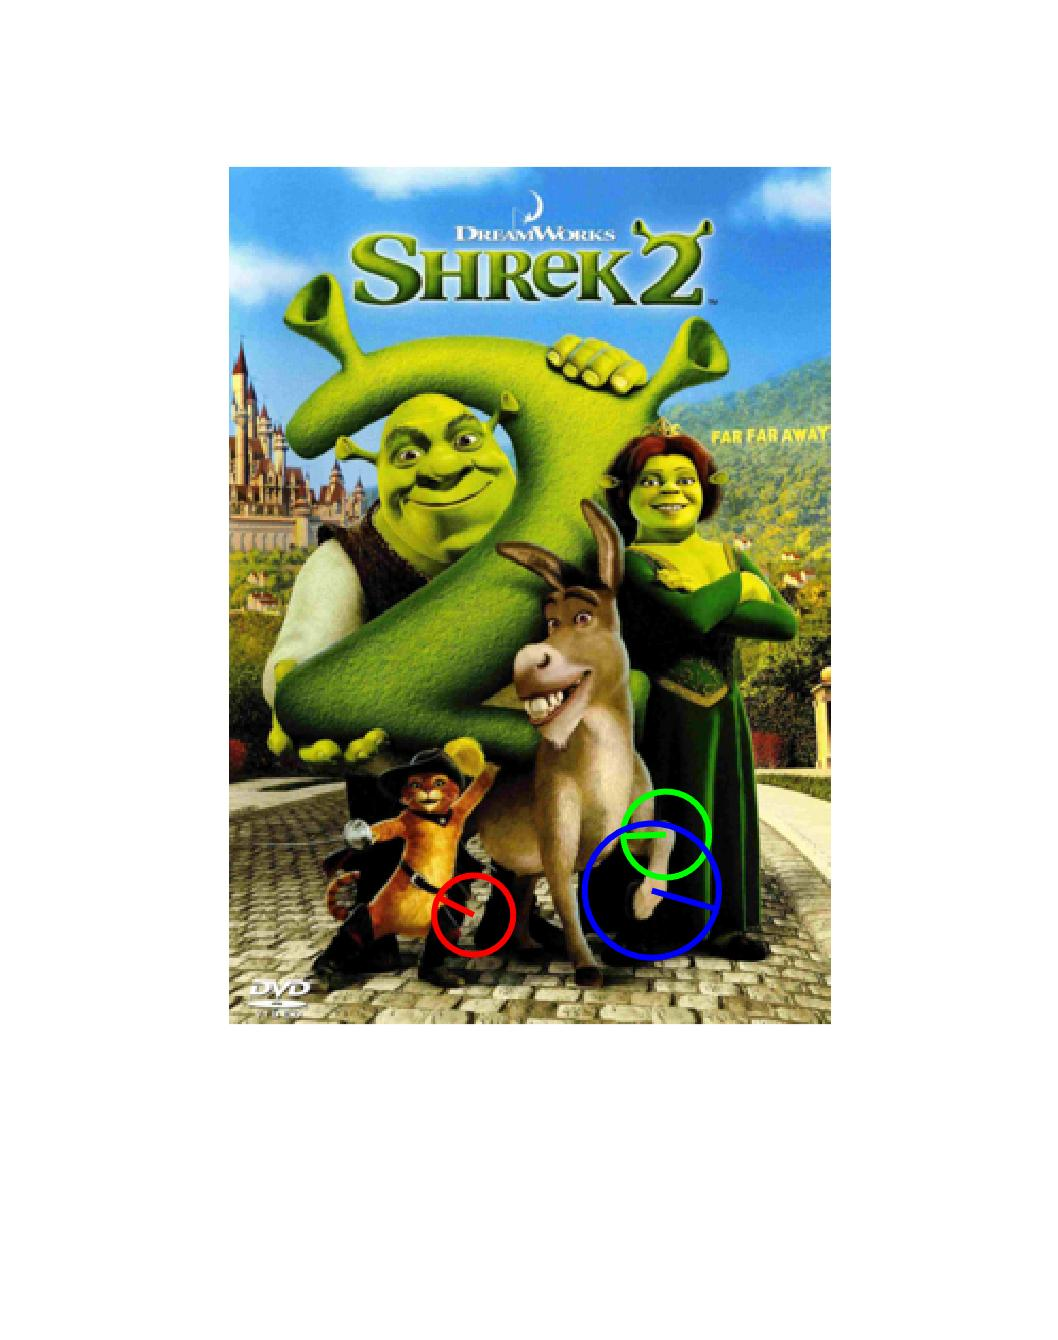
\includegraphics[width=0.7\textwidth, center]{reference_matching.jpg}
\vspace*{-40mm}
\caption{Feature Matching run on reference.png}
\end{figure}
\begin{figure}
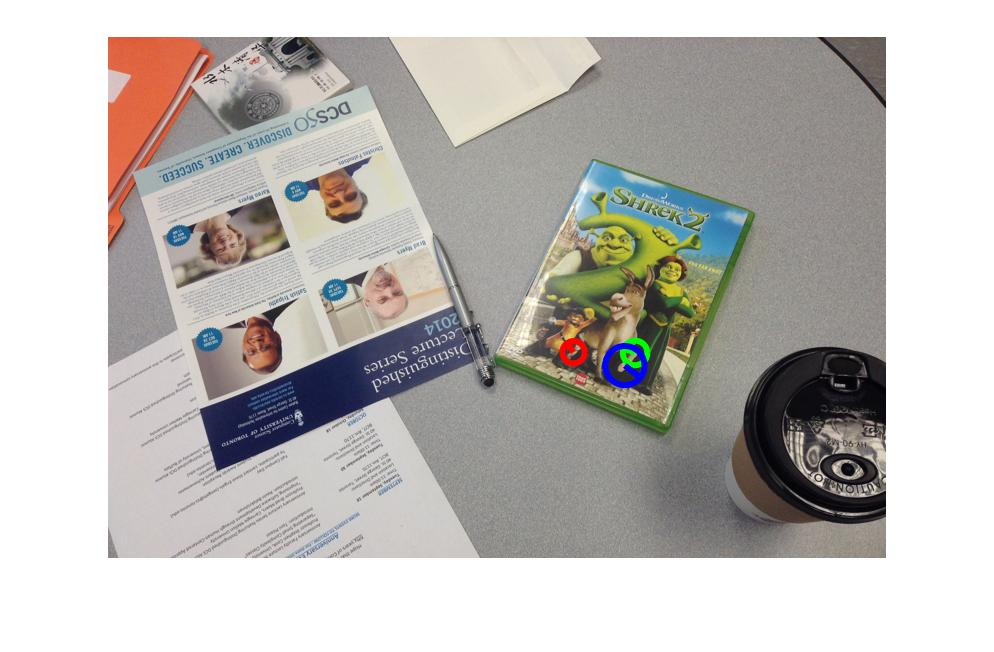
\includegraphics[width=0.7\textwidth, center]{test_matching.jpg}
\vspace{-15mm}
\caption{Feature Matching run on test.png}
\end{figure}
\begin{figure}
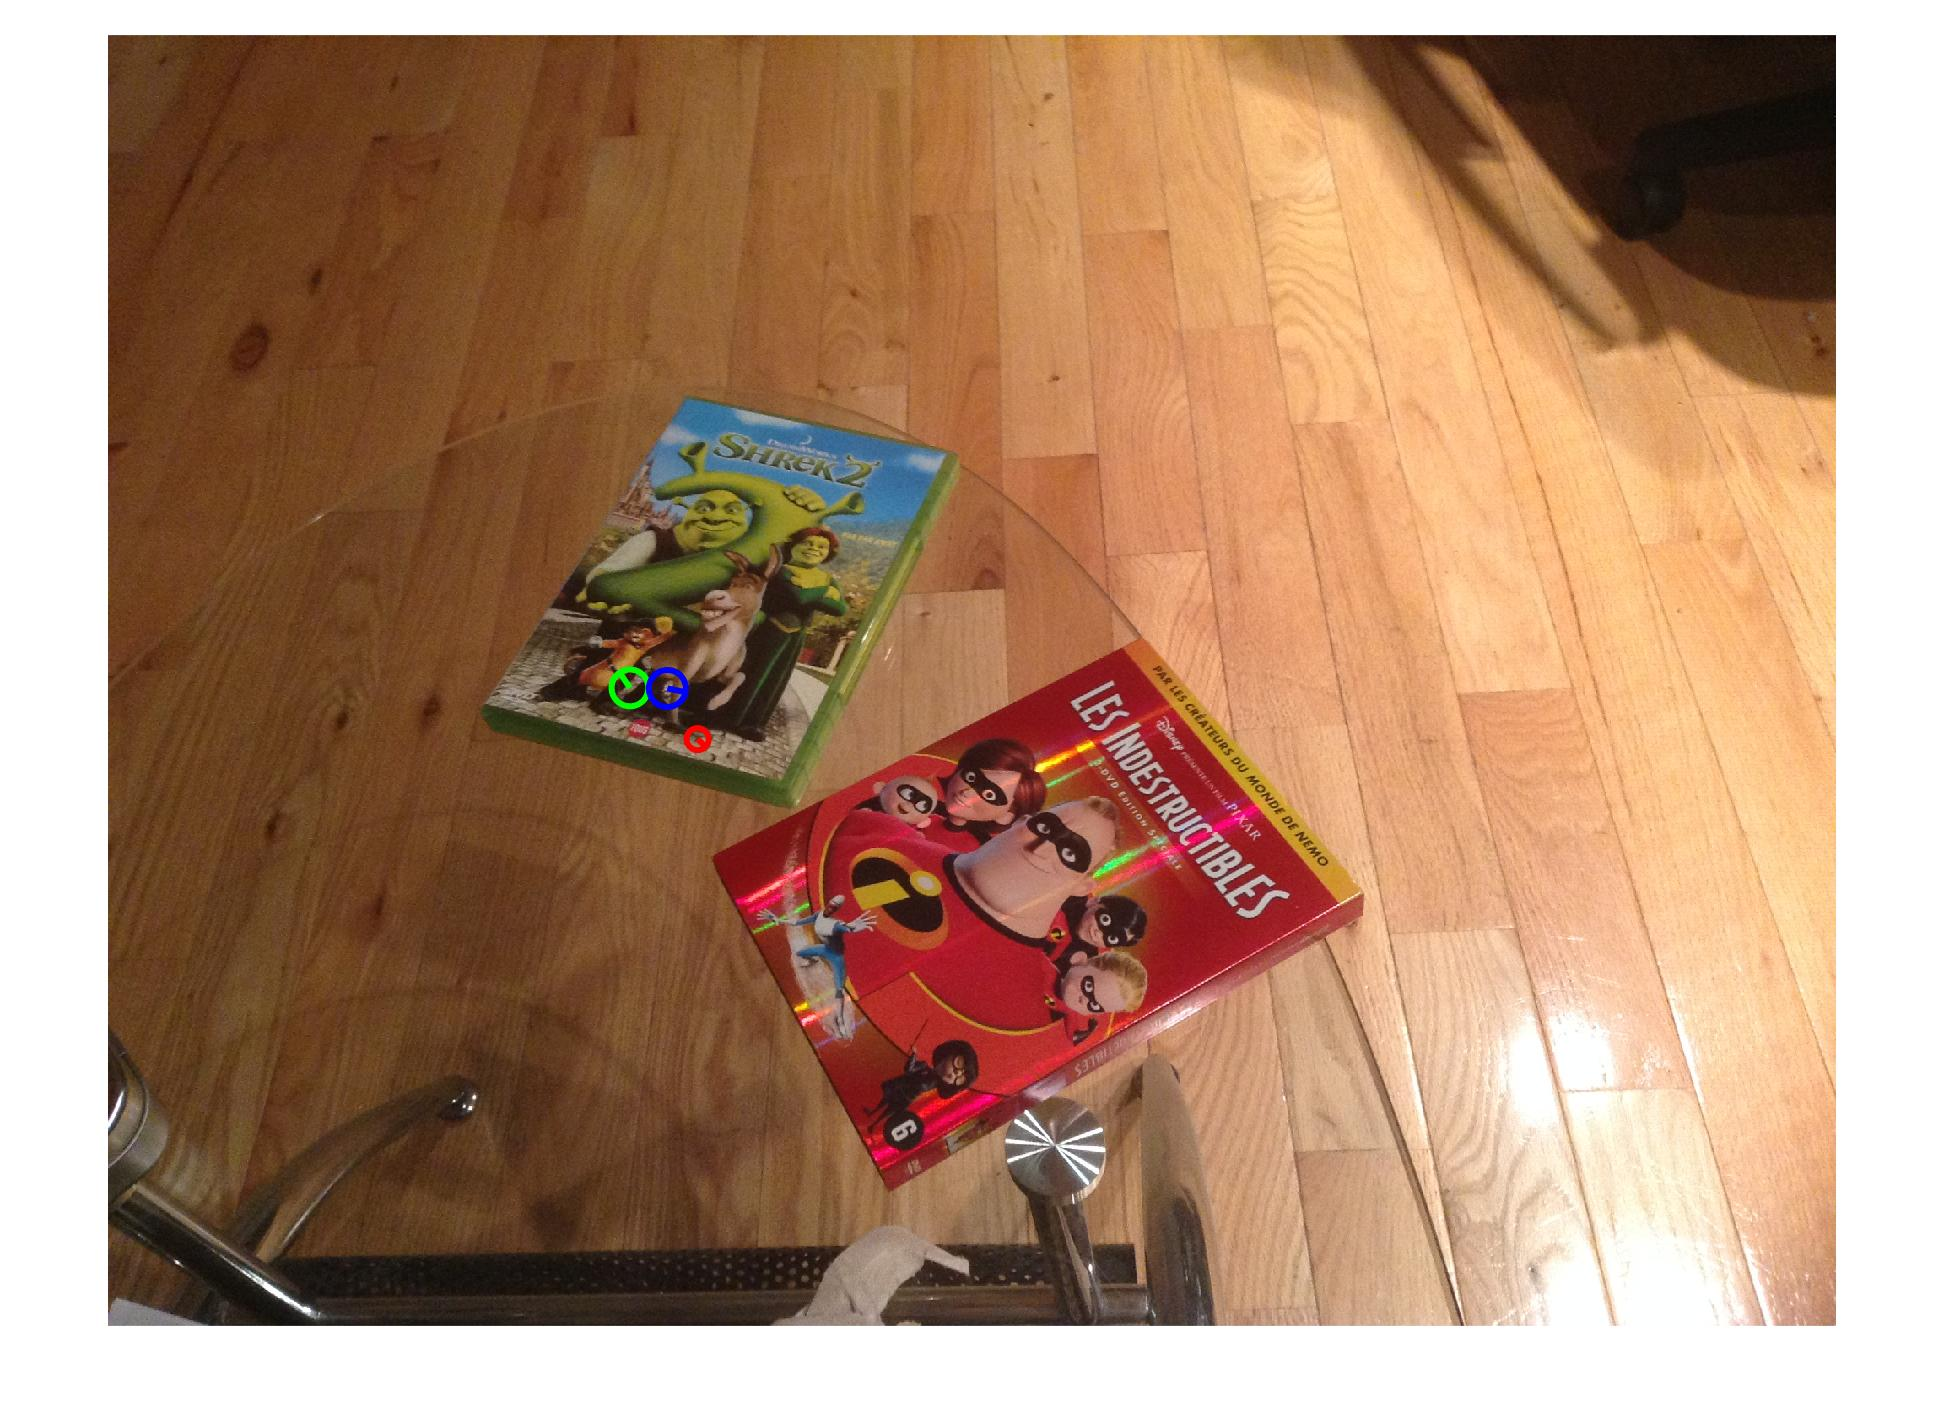
\includegraphics[width=0.7\textwidth, center]{test2_matching.jpg}
\vspace*{-10mm}
\caption{Feature Matching run on test2.png}
\end{figure}
\newpage
\item Affine Transformation: 
\begin{lstlisting}[language=MATLAB]
% affine transformation
function out = a2q2c()
% get top 3 correspondences from a2q2b;
top_3 = a2q2b();

f_ref = top_3('f_ref');
f_test = top_3('f_test');

% keypoints
ref_indices = top_3('ref_indices');
test_indices = top_3('test_indices');

% point matrices
ref_points = [f_ref(1:2, ref_indices(1):ref_indices(1)), f_ref(1:2, ref_indices(2):ref_indices(2)), f_ref(1:2, ref_indices(3):ref_indices(3))];
test_points = [f_test(1:2, test_indices(1):test_indices(1)), f_test(1:2, test_indices(2):test_indices(2)), f_test(1:2, test_indices(3):test_indices(3))];

% since we have 3 keypoints, we use a = inv(P) * P'
P = [];
for i = 1:3
    r1 = [ref_points(1, i), ref_points(2, i), 0, 0, 1, 0];
    r2 = [0, 0, ref_points(1, i), ref_points(2, i), 0, 1];
    P = [P; r1; r2];
end

P_prime = [test_points(1,1); test_points(2,1); test_points(1,2); test_points(2,2); test_points(1,3); test_points(2,3)];

out = P\P_prime;
end
\end{lstlisting}

\item Visualize affine transformation:
\begin{lstlisting}[language=MATLAB]
% Visualize affine
function out = a2q2d()
% read image
im_ref = imread('reference.png');
im_test = imread('test2.png');
[imrows, imcols, ~] = size(im_ref);

% Matrix P 
P = [1, 1, 0, 0, 1, 0; 0, 0, 1, 1, 0, 1;
1, imrows, 0, 0, 1, 0; 0, 0, 1, imrows, 0, 1;
imcols, 1, 0, 0, 1, 0; 0, 0, imcols, 1, 0, 1;
imcols, imrows, 0, 0, 1, 0; 0, 0, imcols, imrows, 0, 1;]

% affine transformation
transformed = a2q2c();
a = P*transformed;

% Plot corners of shrek 2
figure;
imshow(im_test);
hold on;
line([a(1), a(3)],[a(2),a(4)],'color','r', 'linewidth', 3);
line([a(1), a(5)],[a(2),a(6)],'color','r', 'linewidth', 3);
line([a(3), a(7)],[a(4),a(8)],'color','r', 'linewidth', 3);
line([a(5), a(7)],[a(6),a(8)],'color','r', 'linewidth', 3);
hold off;
end
\end{lstlisting}
\begin{figure}
\vspace{-20mm}
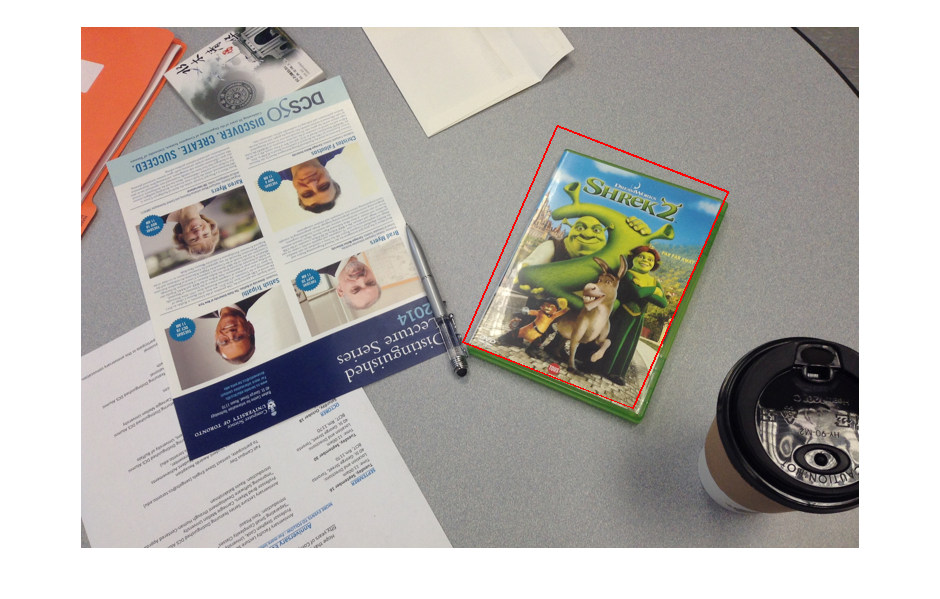
\includegraphics[width=0.7\textwidth, center]{test_affine.png}
\vspace{-10mm}
\caption{Visualize affine transformation on test.png}
\end{figure}
\begin{figure}
\vspace{-10mm}
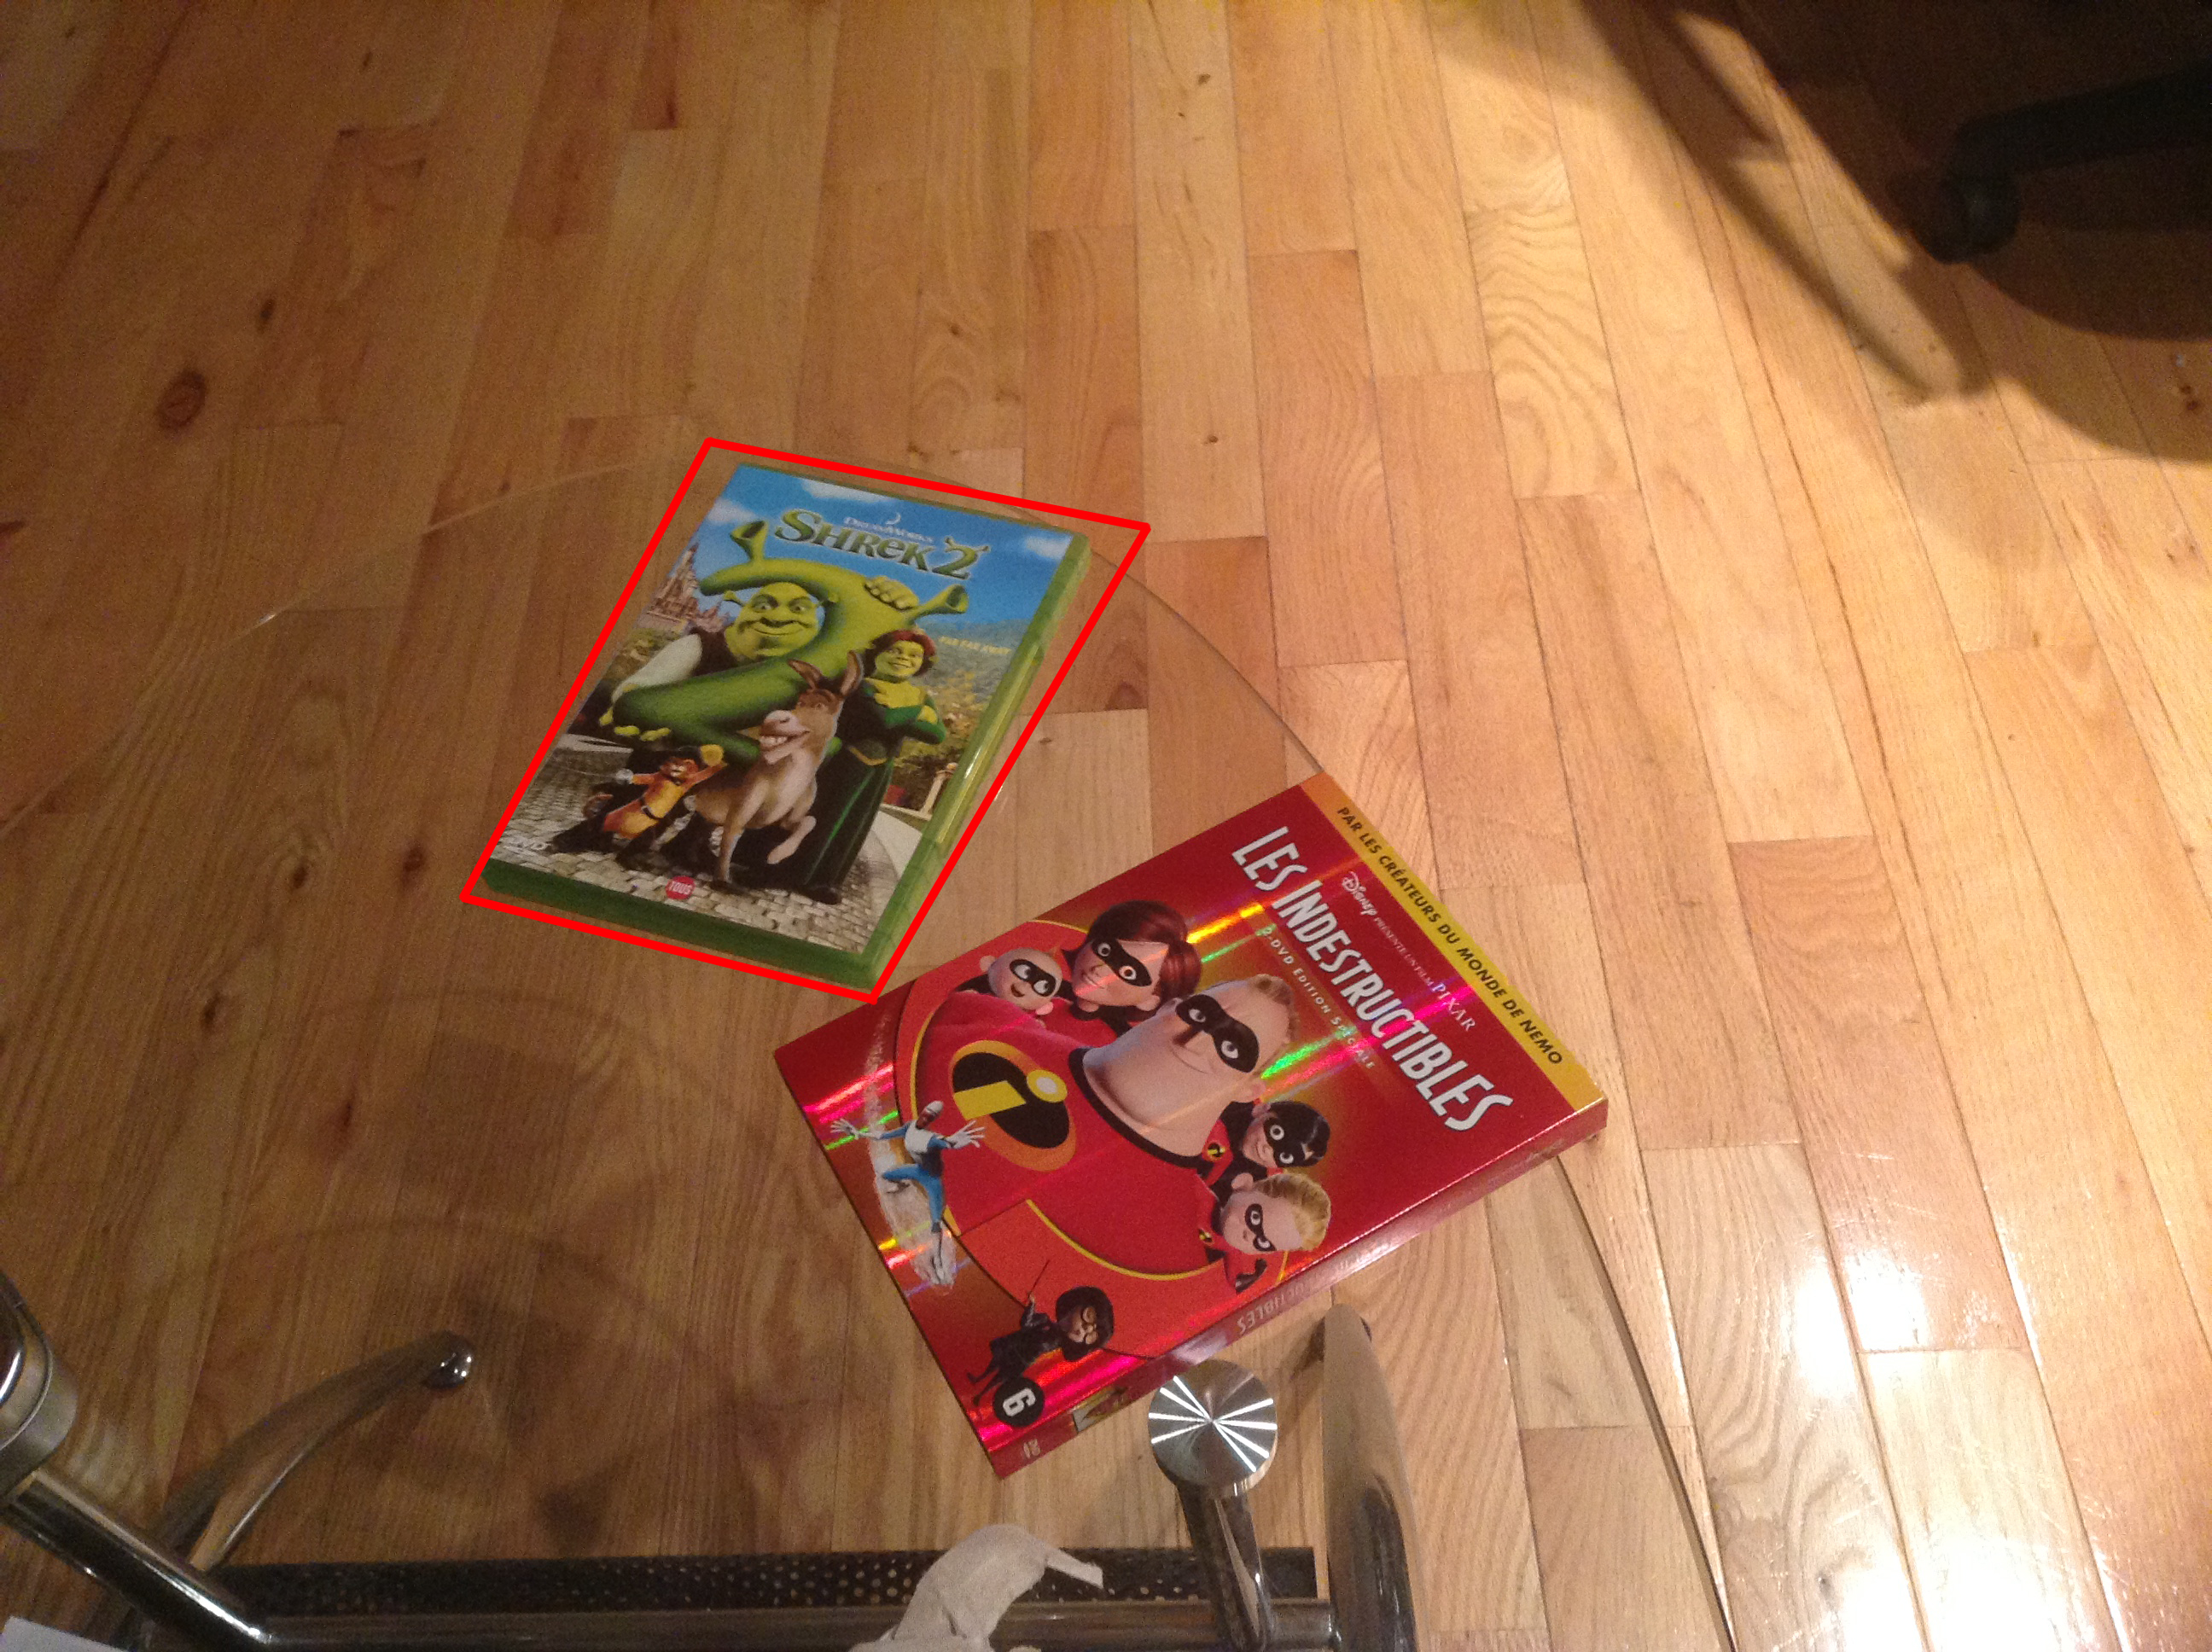
\includegraphics[width=0.7\textwidth, center]{test2_affine.jpg}
\vspace{-5mm}
\caption{Visualize affine transformation on test2.png}
\end{figure}
\end{enumerate}

\newpage
\item[Q3.]
Extra Credit:
\begin{lstlisting}[language=Python]
import numpy as np
import cv2

# load the image, convert it to grayscale, and blur it using gaussian
image = cv2.imread("building_6.jpg")
gray = cv2.cvtColor(image, cv2.COLOR_BGR2GRAY)
gray = cv2.GaussianBlur(gray, (3, 3), 0)

# detect edges in the image using canny
edged = cv2.Canny(gray, 310, 500)
cv2.imshow("Edged", edged)
cv2.waitKey(0)

# detect lines aligned to horizontal and vertical axes using houghLines
lines = cv2.HoughLinesP(edged, 1, np.pi/180, 10, 0, 0)
for x in range(0, len(lines)):
    for x1,y1,x2,y2 in lines[x]:
        cv2.line(image, (x1,y1), (x2,y2), (0,255,0), 2)


cv2.imshow('building',image)
cv2.waitKey(0)
\end{lstlisting}
***OUTPUT ON NEXT PAGE***
\newpage
\begin{figure}
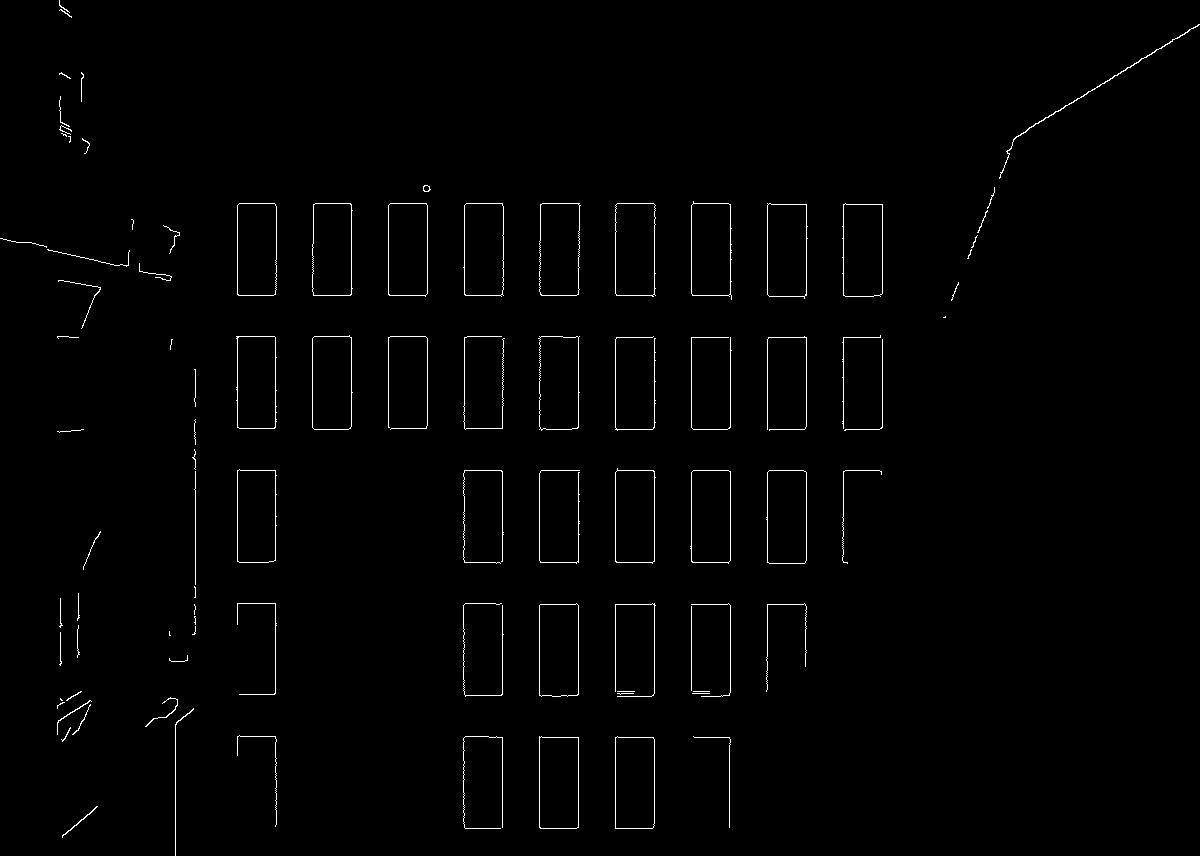
\includegraphics[width=0.7\textwidth, center]{building_6_canny.jpg}
\caption{Ran canny edge detector on building\textunderscore6.jpg}
\end{figure}
\begin{figure}
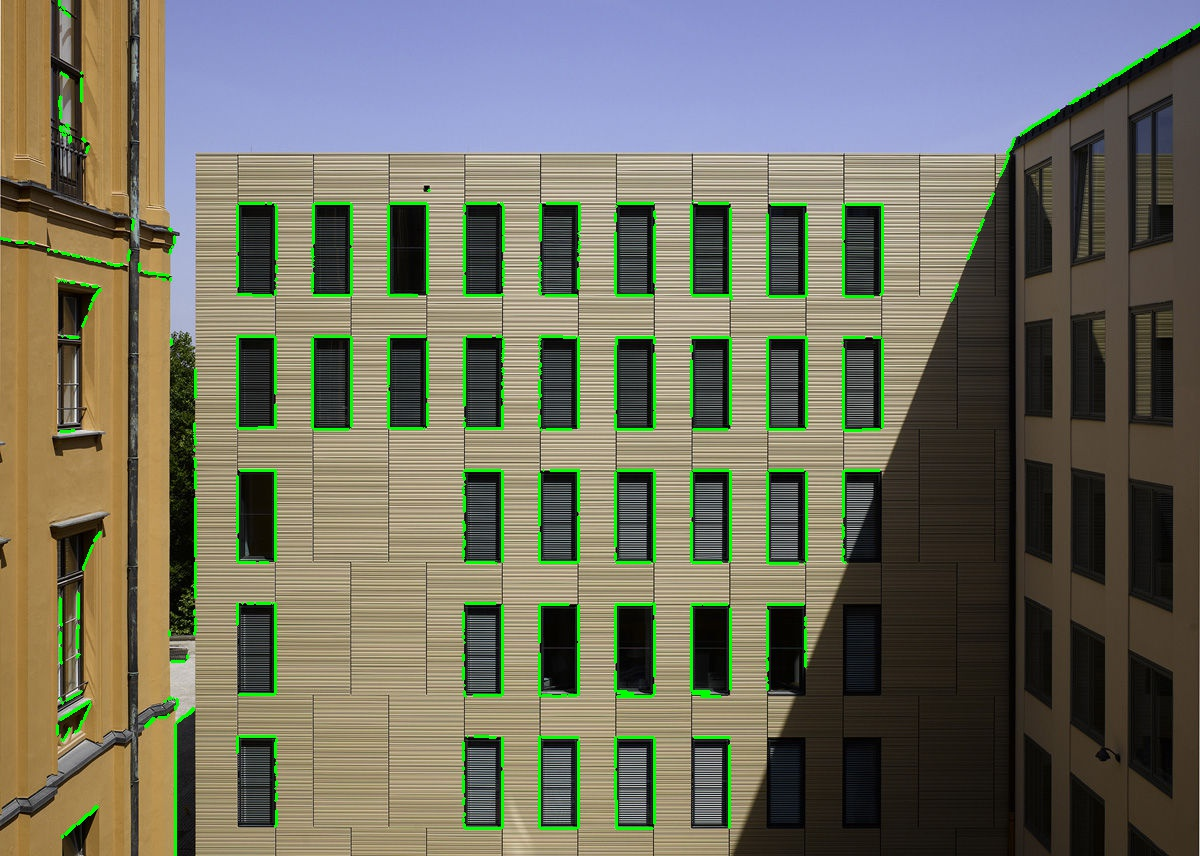
\includegraphics[width=0.7\textwidth, center]{building_6_windows.jpg}
\vspace{-5mm}
\caption{Visualize windows on building\textunderscore6.jpg}
\end{figure}
\begin{figure}
\vspace{-20mm}
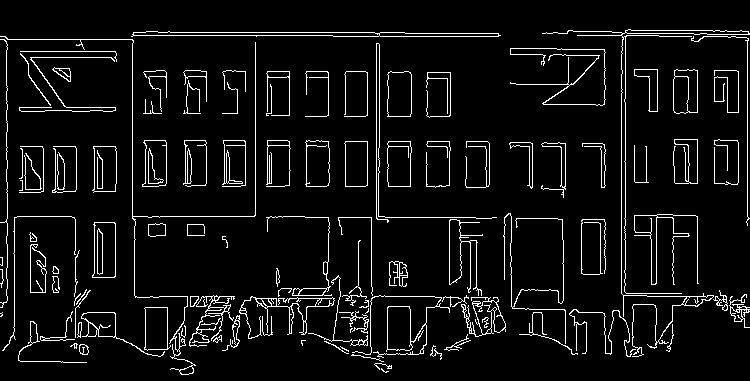
\includegraphics[width=0.7\textwidth, center]{building_3_canny.jpg}
\caption{Ran canny edge detector on building\textunderscore3.jpg}
\end{figure}
\begin{figure}
\vspace{-20mm}
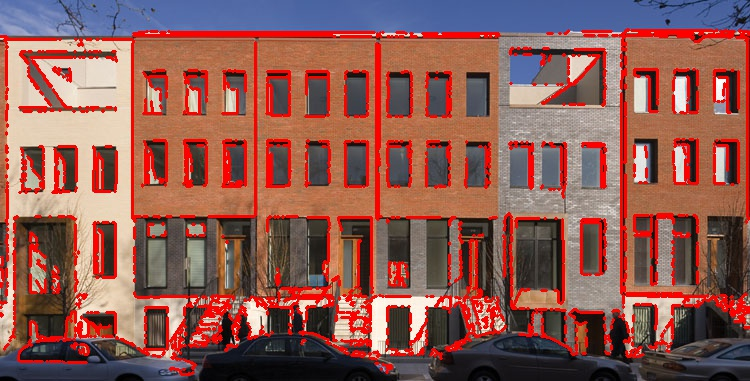
\includegraphics[width=0.7\textwidth, center]{building_3_windows.jpg}
\caption{Visualize windows on building\textunderscore3.jpg}
\end{figure}
\end{description}
\end{document}
  
  



